\documentclass[11pt]{article}

\usepackage[margin=1in]{geometry}
\usepackage[T1]{fontenc}
\usepackage{lmodern}
\usepackage{amsmath,amssymb,amsthm}
\usepackage{mathtools}
\usepackage{enumitem}
\usepackage{tikz}
\usetikzlibrary{arrows.meta,positioning,calc}
\usepackage[hidelinks]{hyperref}
\usepackage{microtype}

\theoremstyle{plain}
\newtheorem{theorem}{Theorem}
\renewcommand{\thetheorem}{\Alph{theorem}}
\newtheorem{proposition}{Proposition}
\newtheorem{lemma}{Lemma}
\newtheorem{corollary}{Corollary}
\theoremstyle{definition}
\newtheorem{definition}{Definition}
\newtheorem{remark}{Remark}

\newcommand{\Exec}{\mathrm{Exec}}
\newcommand{\obs}{\mathrm{obs}}
\newcommand{\Zstar}{Z^{\star}}
\newcommand{\kO}{\kappa_{O}}
\newcommand{\Real}{\mathbb{R}}
\newcommand{\Y}{\mathcal{Y}}
\newcommand{\Sig}{\mathcal{S}}
\newcommand{\Mset}{\mathcal{M}}
\newcommand{\Gates}{\mathcal{B}}
\newcommand{\Defn}[1]{\emph{#1}}

\title{\textbf{A Policy--Coverage Duality for Fungal PKS}\\[2pt]
\large Reducing genome-to-structure prediction to operator soundness: the duality (proven),\\ the floor (characterized), the loop (sound, not shown convergent), the open step (the map's hard families)}
\author{Brage Eilertsen\\ \small brageei@uio.no \quad University of Oslo}
\date{Working note, May 2026 \quad\small(Paper III seed --- to be hardened)}

\begin{document}
\maketitle

\begin{abstract}
The design paper recast fungal polyketide prediction as inference over latent programs $y=\Exec_\Theta(z;G)$, with an identifiability--controllability duality: prediction ambiguity and design freedom are one quantity $\kO$ (Theorem~1, Eilertsen 2026a). The map paper gave a coverage census and a sound-expressibility criterion --- an operator is buildable iff its formula-invariant DOF is a computable function of recoverable $\varphi(B)$ --- and found that $86\%$ of in-scope cores touch a family whose sound expressibility is \emph{unknown} (Eilertsen 2026b). \textbf{This note does not solve fungal PKS and does not claim a near-solution.} It \emph{reduces} the problem and characterizes what a solution would require. Proven: (i) \textbf{$\kO$ factorizes} (Theorem~A) into an exact additive ledger over typed gates, so hardness is per-gate and the training loss is counted in gates, not clusters; (ii) \textbf{expressibility and learnability are dual} (Theorem~B, the central contribution) --- learning the per-cycle policy (cycle scale) and extending the operator grammar (operator scale) are one predicate, $d(b)\in\mathrm{image}(\varphi)$, both bottoming out at Rung~4 (their finer relation is contingent, Rem.~\ref{rem:floor}); (iii) the wake--sleep loop built on these is \textbf{unconditionally sound} (Proposition~\ref{prop:sound}). The honest negative space, stated as such: the loop's coverage-growth step \emph{is} the map's open problem, not a subroutine (Lemma~\ref{lem:order}); $\mathcal{K}$-descent is \emph{conditional} on the exchange rate $\lambda$ (Proposition~\ref{prop:descent}); convergence to the floor is \emph{open} and equals the coverage question (Remark~\ref{rem:conv}); and the floor's narrowness is itself conditional on a structure-to-kinetics chain we cannot here verify. The contribution is therefore a reduction (solve-fungal-PKS $\Rightarrow$ supply the rungs of the soundness-open families), the policy/coverage duality, a \emph{characterized} (not attained) floor, and four falsifiable predictions --- chiefly P1, a Gate-3-specific accuracy lift, absent at Gate-2, whose non-differential appearance would falsify the rung assignment.
\end{abstract}

\section{The one-function reduction (inherited, sharpened)}
A program is a cycle list $z=(c_t,a_t)_{t=1}^N$ rendered left-to-right by a sound deterministic executor $\Exec_\Theta(\cdot;G):\mathcal{Z}(G)\to\Y$; an observable set $O$ projects structures to signatures $\obs_O:\Y\to\Sig$, and $\varphi_O=\obs_O\circ\Exec_\Theta$ is the observable map of a program. The verifier returns the consistent set $\Zstar(z;O)=\{z'\,:\,\varphi_O(z')=\varphi_O(z)\}=[z]_O$, with $\kO(z)=\lvert[z]_O\rvert$ (Theorem~1, 2026a).

The outlook of 2026a frames the iterative synthase as a partially observed deterministic control system with four objects: the transition $s_{t+1}=F(s_t,a_t)$, the emission $y=\mathrm{readout}(s_N)$, the posterior $\Zstar$, and the per-cycle policy $\pi(a\mid s_t,\varphi(G))$. \emph{Three are known exactly}: $F$ is the executor (applying an operator to the ACP-tethered intermediate \emph{is} $F$), the emission is the readout, $\Zstar$ is the verifier. Direct $\text{BGC}\!\to\!\text{structure}$ regression stalled at $51\text{--}68\%$ because it learned the whole composition end-to-end from terminal data; the executor returns three factors and leaves one. We take this as the starting point --- with a caveat the map paper forces and that this note keeps central: the reduction holds \emph{only over a fixed grammar}. ``Solving fungal PKS'' is system identification of a single policy $\pi$ \emph{plus} extension of the grammar to cover the deposited manifold, and the second half is the map's open problem (\S\ref{sec:order}, \S\ref{sec:limits}). The rest of this note makes both precise and is careful to prove only what survives \emph{around} the open step, not the step itself.

\section{Theorem A: the hardness factorizes over typed gates}
\label{sec:kfac}
Because $\Exec_\Theta$ renders programs left-to-right and is deterministic, the consistent set is prefix-closed: $\Zstar(y;O)$ is exactly the leaf set of a finite rooted tree $T(y;O)$ --- the \Defn{program trie} --- whose depth-$t$ edges are the per-cycle actions $a_t$ retained after $O$-pruning (this is the prefix trie of \S15, 2026a, and its branch points are the Gates of the Outlook). Let $\Gates(y;O)$ be the internal nodes of $T$ with $\geq 2$ children (the \Defn{gates}), and for a gate $b$ let $\deg(b)$ be its number of surviving children.

\begin{theorem}[$\kO$-factorization]\label{thm:kfac}
For every product $y$ reachable under $(G,\Theta)$ and observable set $O$,
\begin{equation}
\kO(y)\;=\;1+\sum_{b\in\Gates(y;O)}\bigl(\deg(b)-1\bigr).
\label{eq:kfac}
\end{equation}
Consequently $\kO(y)=1$ (the product is exactly identified, and by Theorem~1 exactly specified for design) \emph{iff} $T(y;O)$ has no gates: every cycle's action is forced by the prefix and the observables.
\end{theorem}

\begin{proof}
$\Zstar=[z]_O$ equals the leaf set of $T$ by prefix-closedness and the verifier's soundness and relative completeness (\S4.1, 2026a): every returned program executes to a structure $\simeq y$ and every legal such program is returned, so the retained edges are exactly the $O$-consistent continuations. For any finite rooted tree the number of leaves equals $1+\sum_{v}(\deg(v)-1)$ summed over internal nodes, and internal nodes with a single child contribute $0$; restricting the sum to multi-child nodes gives \eqref{eq:kfac}. The $\kO=1$ characterization is immediate.
\end{proof}

\noindent\textbf{What is new.} Theorem~1 (2026a) gives $\kO$ as a cardinality; Theorem~A makes it an \emph{exact additive ledger over typed gates}. Each gate inherits the Outlook's type: a \Defn{Gate-2} (candidates differ in a per-cycle reduction label, resolvable by a running substrate count --- the Substrate-Prefix Engine of \S11) or a \Defn{Gate-3} (candidates share a reduction trajectory and differ only in the mass-neutral position of a C-methylation --- label-symmetric, requiring the Geometric-Rescue Engine). Equation~\eqref{eq:kfac} says the field's hardness at $y$ is literally the sum of its gates, and ``resolving $y$'' is closing them one by one. The empirical shape measured in \S15 of 2026a --- Gate-3 absent over non-methylating aromatics, single-digit within HR, concentrated in small methylating clusters --- is now the \emph{statement that the Gate-3 terms of \eqref{eq:kfac} are sparse and localized}, i.e.\ the residual sum is short.

\begin{remark}[the ledger is the loss]
The marginal-likelihood objective $\mathcal{L}(\theta)=-\sum_B\log\sum_{z\in\Zstar(B)}\pi_\theta(z\mid B)$ factorizes over the common prefix of $\Zstar$ (\S15, 2026a); under \eqref{eq:kfac} it factorizes over exactly the gates of $T$. A clean trunk edge is a \emph{free, correct} per-cycle label manufactured by the executor; only gate edges carry a learning signal. Training data is therefore counted in \emph{gates}, not clusters --- the quantitative engine of \S\ref{sec:loop}.
\end{remark}

\section{Theorem B: expressibility and learnability are one criterion at two scales}
\label{sec:dual}
A gate $b$ has a \Defn{branch-selecting DOF} $d(b)$: which surviving child is the true continuation. Closing $b$ means computing $d(b)$ from recoverable features. The map paper's criterion (\S6, 2026b) --- an operator $O$ is soundly expressible from $\varphi$ iff its formula-invariant DOF is a computable function of $\varphi(B)$ --- is the \emph{same predicate} applied to $d(b)$, and the map paper's cost ladder classifies \emph{which coordinate of $\varphi$ supplies it}:
\begin{description}[leftmargin=2.4em,itemsep=1pt]
\item[Rung 1] $d(b)=f(s_t)$: the substrate prefix alone (label-distinguishable Gate-2; \emph{free}).
\item[Rung 2] $d(b)=f(s_t,\text{seq})$: a sequence-keyed rule (ESM head; per-module bacterial sequence; PT-clade regiochemistry).
\item[Rung 3] $d(b)=f(s_t,\text{fold/dynamics})$ but not sequence directly: recoverable through $\text{AF2}:\text{seq}\to\text{fold}$ and $\text{MD/QM}:\text{fold}\to\text{kinetics}$ (label-symmetric Gate-3; \emph{costly, but a function}).
\item[Rung 4] $d(b)$ is not a function of any cluster feature: an intrinsic mixture (a within-enzyme collision: one sequence, one substrate, $\geq 2$ products) or an extra-genomic determinant. \emph{No function exists.}
\end{description}

A gate may be \Defn{in-grammar} (its true child is present in $T$, awaiting selection --- the policy's job) or a \Defn{boundary gate} (the true child is absent because $\Theta$ cannot express the operator --- coverage's job: admit the branch, \emph{then} select). This is the only structural difference between the two scales.

\begin{theorem}[expressibility--learnability duality]\label{thm:dual}
Fix $(G,\Theta,O)$. Define the residual-DOF set
\[
\Delta(G,\Theta,O)\;=\;\{\,d(b)\,:\,b\ \text{a gate, in-grammar or boundary, with }\mathrm{rung}(b)\ \text{not yet supplied}\,\}.
\]
Write $\Delta^{\mathrm{pol}}_\varphi$ and $\Delta^{\mathrm{cov}}_\varphi$ for the in-grammar gates the policy cannot resolve and the boundary operators coverage cannot express at budget $\varphi$; both are readouts of the one predicate $d(b)\in\mathrm{image}(\varphi)$ --- closing a gate (policy) and expressing an operator (coverage) alike. \emph{Over the information operator} $I_\varphi(b)=\mathbf{1}[d(b)\in\mathrm{image}(\varphi)]$ both residuals shrink monotonically as $\varphi$ climbs, since $\mathrm{image}(\varphi)$ only grows; the finite-sample empirical error need not (Rem.~\ref{rem:infovsemp}). \emph{Invariant (proven):} the limits $\Delta^{\mathrm{pol}}_\infty$ and $\Delta^{\mathrm{cov}}_\infty$ consist entirely of Rung-4 obstructions --- $d(b)$ a function of no cluster feature --- which no feature budget removes. \emph{Topology (contingent):} their relation --- shared core, containment, or incomparability --- is fixed by the executor's representation of non-functional steps (Rem.~\ref{rem:floor}), a design choice over case populations not yet instantiated in the corpus.
\end{theorem}

\begin{proof}[Proof sketch]
By Theorem~A the policy's only learnable targets are the in-grammar gates; its irreducible error is the entropy of those $d(b)$ not determined by $\varphi$, zero exactly when $\varphi$ contains each gate's rung coordinate (the criterion of \S6, 2026b, read at cycle scale). Operator coverage adds a boundary gate's true child iff that operator's formula-invariant DOF is a function of $\varphi$ --- the same criterion read at operator scale. Both predicates are ``$d(b)\in\mathrm{image}(\varphi)$'', monotone under enlarging $\varphi$ \emph{over the information operator} $I_\varphi$ (a larger feature set cannot make a previously-expressible DOF inexpressible, since the policy may ignore coordinates; the finite-sample error is a separate matter, Rem.~\ref{rem:infovsemp}). Rung~4 is precisely the case where $d(b)$ is not a function of \emph{any} cluster feature --- an intrinsic distribution has no point target, an extra-genomic determinant is outside $\varphi$ by definition --- so it lies in neither image at any budget. The invariant is all the proof delivers; the relation between the two limit sets is settled below, not here.
\end{proof}

\begin{remark}[information operator vs.\ empirical error]\label{rem:infovsemp}
Theorem~B's monotonicity is a statement about $I_\varphi$ --- whether $d(b)$ is closable \emph{in principle} at budget $\varphi$. The quantity P1/P2 measure is the \emph{empirical} held-out error, which decomposes as an approximation term (monotone non-increasing in $\mathrm{image}(\varphi)$) plus an estimation term that can \emph{rise} with feature dimension. Adding the high-dimensional AF2 pose trajectory can therefore increase held-out error on a gate a leaner $\varphi$ already closed, with the information still present. P1 is thus a claim about the approximation term, to be read with capacity control or in the data-rich regime; a variance-driven bump is not a falsification.
\end{remark}

\begin{remark}[the Rung-4 floor: four populations, presently uninstantiated]\label{rem:floor}
Enumerating what can be Rung-4 gives four populations. $A(\mathrm{i})$: a genuine mixture with both products buildable --- the verifier returns $\kO\ge 2$ \emph{and} no sound function exists, so it sits on \emph{both} floors (the shared core). $A(\mathrm{ii})$: extra-genomic routing among buildable children --- irreducible $\kO$ but no missing operator, hence \emph{policy floor only}. $B$: a Rung-4 operator whose true child is unbuildable while its gate still surfaces in-grammar via other children --- \emph{coverage floor only} (Lemma~\ref{lem:order}). $C$: a Rung-4 operator occurring only inside otherwise-out-of-grammar programs, never surfacing in-grammar --- \emph{coverage floor only}. Thus $\Delta^{\mathrm{pol}}_\infty=\{A(\mathrm{i}),A(\mathrm{ii})\}$ and $\Delta^{\mathrm{cov}}_\infty=\{A(\mathrm{i}),B,C\}$: incomparable in general; containment $\Delta^{\mathrm{pol}}_\infty\subseteq\Delta^{\mathrm{cov}}_\infty$ iff $A(\mathrm{ii})=\varnothing$; equality iff also $B=C=\varnothing$; set-identity (the discarded ``identical'' claim) iff both wings vanish. Two construction facts decide which holds. \textbf{Q1:} can a Rung-4 gate occur only in out-of-grammar programs ($C$)? \textbf{Q2:} does the executor represent a non-functional step as one in-grammar gate with $\kO\ge 2$ (policy side) or exclude it by a soundness-requires-a-function rule (coverage side), and is $\Delta^{\mathrm{cov}}$ indexed by missing buildable children or by missing sound functions? Both are \emph{design decisions over case populations not yet instantiated}: the corpus holds no confirmed Rung-4 core, so $A(\mathrm{ii}),B,C$ are presently empty and even $A(\mathrm{i})$ is unconfirmed (zero verified within-enzyme collisions). The invariant is proven; the topology is a statement about possibly-vacuous sets, resolved by construction choices not yet pinned --- and if no $A(\mathrm{i})$ is ever confirmed the floor is itself empty, which is its own finding: Rung~4 conjectured, never demonstrated.
\end{remark}

\noindent This is the companion to Theorem~1 (2026a). Theorem~1: \emph{predict} $\leftrightarrow$ \emph{design} are one $\kO$. Theorem~B: \emph{learn-policy} $\leftrightarrow$ \emph{extend-grammar} share one predicate $d(b)\in\mathrm{image}(\varphi)$ and a Rung-4 floor-character, with two (in general incomparable) residuals (Rem.~\ref{rem:floor}). And the two dualities are the \emph{same statement at two scales} of the program grammar, summarized in Table~\ref{tab:master}: one predicate, ``is the hidden DOF a computable function of recoverable $\varphi$?'', governs all four corners.

\begin{table}[h]
\centering
\small
\begin{tabular}{l|cc}
 & \textbf{inference question} & \textbf{action question}\\\hline
\textbf{cycle scale} (a gate $d(b)$) & predict the per-cycle action & specify/edit the iteration program\\
 & \multicolumn{2}{c}{$\downarrow$ one quantity $\kO$ (Thm.~1) $\downarrow$}\\[2pt]
\textbf{operator scale} (an operator DOF) & is this product reconstructible? & is this operator buildable?\\
 & \multicolumn{2}{c}{$\downarrow$ one set $\Delta$ (Thm.~B) $\downarrow$}\\\hline
\textbf{closes by} & \multicolumn{2}{c}{climbing $\varphi=\text{seq}\to\text{fold}\to\text{dynamics}$; floor at Rung 4}
\end{tabular}
\caption{The master $2\times 2$. A single predicate --- $d\in\mathrm{image}(\varphi)$ --- governs prediction, design, policy learning, and operator coverage. Theorem~1 unifies the top row's columns; Theorem~B unifies the rows; the rung ladder supplies the common closing mechanism.}
\label{tab:master}
\end{table}

\section{Lemma 1: coverage strictly precedes policy}
\label{sec:order}
\begin{lemma}[coverage-gates-policy]\label{lem:order}
If the in-vivo program $z^\star$ of a target $y$ is out-of-grammar, $z^\star\notin\mathcal{Z}(G)$, then $z^\star\notin\Zstar(y;O)$ for every $O$, so no policy $\pi$ ranking within $\Zstar$ can return $z^\star$. Hence on out-of-grammar cores the marginal value of any policy is zero, and operator extension is a strict prerequisite.
\end{lemma}
\begin{proof}
$\Zstar(y;O)\subseteq\mathcal{Z}(G)$ by construction; $z^\star\notin\mathcal{Z}(G)$ gives $z^\star\notin\Zstar$. A policy is a reweighting of $\Zstar$, whose support excludes $z^\star$.
\end{proof}

\noindent\textbf{Citrinin is the worked instance.} In \S11 (2026a) the geometric-rescue head drove held-out entropy to $0.01$ and committed $\sim$99.9\% mass to a single in-grammar candidate --- yet the true biology requires two C-methylation events, an \emph{out-of-grammar} program at that formula. The entropy collapse proves the structural channel carries discriminating information (the policy is real); Lemma~\ref{lem:order} explains why it nonetheless selected the wrong subtree (the truth was off the trie). The moral is an \emph{ordering} on the loop of \S\ref{sec:loop}: spend on coverage until a core's true program is in-grammar; only then does policy resolution of its gates mean anything. Confident closure of an in-grammar gate on an under-covered core is the failure mode to guard against, and it is detectable --- a verified verdict that the metabologenomics triage of \S9 (2026a) would route to expression$+$NMR.

\section{The loop: a sound, self-funding scaffold around an open step}
\label{sec:loop}
Theorems~A--B and Lemma~\ref{lem:order} assemble into one procedure (Figure~\ref{fig:loop}), a literal wake--sleep instantiation of the execution-guided program synthesis the design paper cites (DreamCoder; Ellis et al.\ 2021):

\begin{enumerate}[leftmargin=1.6em,itemsep=1pt]
\item \textbf{Sleep (dream).} The sound executor, run forward as a generator, enumerates producible programs and renders them to structures --- an unbounded synthetic $(\text{structure},\varphi)\!\to\!z$ corpus. Pretrain the shared policy $\pi_\theta$ to invert it. This amortizes the verifier's enumeration into a network and shapes $\pi$ by the chemistry before any real label is seen.
\item \textbf{Wake (verify).} On real clusters the verifier returns $\Zstar$; by Theorem~A its clean trunk supplies free correct per-cycle labels and its gates supply the learning signal. Fine-tune $\pi_\theta$ on these manufactured labels under the factorized marginal-likelihood loss. \emph{One shared $\pi$ for the whole family}: the compression that hides per-step state from a static reader (the very cause of the $0.567$ wall) is what makes all HR-PKS share a single policy, so lovastatin's and citrinin's cycles train the same function --- the curse read as a transfer blessing.
\item \textbf{Abstraction (grow coverage) --- this step \emph{is} the open problem, not a subroutine.} Two extensions, both \emph{verifier-gated}: (a) reusable cycle motifs discovered in $\Zstar$ become library operators (sound by construction); (b) for each hard family the Rung 0--4 instrument (\S6, 2026b) \emph{would} adjudicate a learned, gene-conditioned operator, admitted only if it passes the mass/formula gate \emph{and} a held-out $\simeq$-match. But whether (b) \emph{succeeds} is precisely the map's unsolved question: the instrument has returned exactly one verdict (aromatic cyclization, Rung 2, on closures curated and encoded before the instrument existed), while macrolactonization (Rungs 2--3, unmeasured) and oxidation/rearrangement (unassessed) together touch $86\%$ of in-scope cores. So coverage growth past the eight reachable cores is \emph{conditional on rung assignments that are open}; by Theorem~B's own logic, if those families are Rung~4 the loop provably cannot reach them. The loop is well-defined and sound (Prop.~\ref{prop:sound}) over families whose rung is established; over the rest it \emph{names} the work, it does not perform it. New operators, where they exist, admit boundary gates' true children (Lemma~\ref{lem:order}), enlarging $\Mset(G)$.
\item \textbf{Direct (the planner is already the controller).} The experiment-selection planner of \S9.5 (2026a) --- by Corollary~1 there already a design planner --- is \emph{also} the loop's controller: it ranks, by expected $\Delta\kO$ per unit cost, both which folds/structures to compute (which $\varphi$-coordinate to buy for which Gate-3 cluster) and which operators to encode next. Because the Gate-3 ledger of Theorem~A is sparse and localized, the structural-data campaign is small and targeted, not a structural-genomics sweep.
\end{enumerate}

Three claims about the loop must be separated, because they have different status; conflating them is how a sound scaffold gets mistaken for a solution.

\begin{proposition}[monotone soundness --- proven, unconditional]\label{prop:sound}
Every iterate of the loop emits only mass/chemistry-consistent, $\simeq$-certified structures. Each learned component is verifier-gated, so its outputs lie in $\Zstar$ intersected with verifier-passing proposals, a subset of the sound set (\S4.1, 2026a). Soundness is therefore invariant along the loop, with no condition on $\varphi$, on $\lambda$, or on the coverage question.
\end{proposition}

\begin{proposition}[$\mathcal{K}$-descent --- conditional on $\lambda$]\label{prop:descent}
Under policy improvement at fixed membership the in-grammar ledger of \eqref{eq:K} is non-increasing (per-core $\kO$ is a $\min$ over a superset of decision rules as $\varphi$ climbs), and coverage is append-only. But admitting a previously out-of-grammar core $y$ moves it from the coverage-gap term into the ledger, changing $\mathcal{K}$ by
\begin{equation}
\Delta\mathcal{K}(y)\;=\;\log\kO(y)\;-\;\lambda\,c(y),
\label{eq:transfer}
\end{equation}
\emph{unsigned in general}: a newly admitted hard core arrives carrying its own gates, so $\log\kO(y)$ may be large. Hence $\mathcal{K}$ is non-increasing along the loop \emph{iff} $\lambda\,c(y)\ge\log\kO(y)$ for every admitted core --- a condition on $\lambda$, not a theorem. Forcing it with large $\lambda$ has a cost: $\mathcal{K}$ becomes dominated by the coverage-gap count, so ``$\mathcal{K}$ small'' ceases to mean ``predictions are good'' and means only ``few cores remain out-of-grammar.'' The earlier draft asserted unconditional monotonicity; \eqref{eq:transfer} is the term that assertion omitted, and \S\ref{sec:limits}(2) is its counterexample.
\end{proposition}

\begin{remark}[convergence to the floor --- open]\label{rem:conv}
Even where Proposition~\ref{prop:descent}'s condition holds, monotone descent of a bounded-below $\mathcal{K}$ gives convergence to \emph{some} limit, not to $\mathcal{K}_\infty$. Attaining the floor additionally requires that descent not stall above it --- that every above-floor gate is eventually closed and every in-scope family eventually covered at finite cost. That is exactly the map's open coverage question (\S\ref{sec:order}, \S\ref{sec:limits}), not a consequence of the loop's structure. Theorem~B characterizes \emph{where} the floor is ($\Delta_\infty$, Rung 4); nothing here proves the loop \emph{reaches} it. The gap between ``the floor is $X$'' and ``the procedure attains $X$'' is the gap between this note and a solution.
\end{remark}

\begin{figure}[h]
\centering
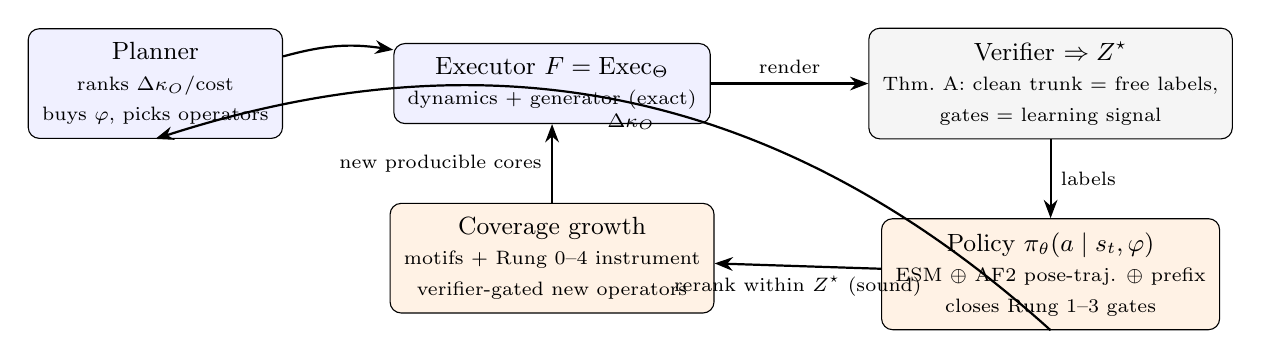
\begin{tikzpicture}[
  >=Stealth, node distance=10mm and 20mm,
  box/.style={draw, rounded corners, align=center, inner sep=5pt, font=\small, minimum height=9mm},
  sym/.style={box, fill=blue!6},
  learn/.style={box, fill=orange!10},
  gate/.style={box, fill=black!4},
  every edge/.style={draw, ->, thick}
]
\node[sym]   (exec)  {Executor $F=\Exec_\Theta$\\ \scriptsize dynamics + generator (exact)};
\node[gate, right=of exec] (ver) {Verifier $\Rightarrow \Zstar$\\ \scriptsize Thm.~A: clean trunk = free labels,\\ \scriptsize gates = learning signal};
\node[learn, below=of ver] (pol) {Policy $\pi_\theta(a\mid s_t,\varphi)$\\ \scriptsize ESM $\oplus$ AF2 pose-traj. $\oplus$ prefix\\ \scriptsize closes Rung 1--3 gates};
\node[learn, below=of exec] (cov) {Coverage growth\\ \scriptsize motifs + Rung 0--4 instrument\\ \scriptsize verifier-gated new operators};
\node[sym, left=14mm of exec] (plan) {Planner\\ \scriptsize ranks $\Delta\kO/\text{cost}$\\ \scriptsize buys $\varphi$, picks operators};

\draw (exec) edge node[above,font=\scriptsize]{render} (ver);
\draw (ver)  edge node[right,font=\scriptsize]{labels} (pol);
\draw (pol)  edge node[below,font=\scriptsize]{rerank within $\Zstar$ (sound)} (cov);
\draw (cov)  edge node[left,font=\scriptsize]{new producible cores} (exec);
\draw (plan) edge[bend left=12] (exec);
\draw (pol.south) edge[bend right=30] node[below,font=\scriptsize]{$\Delta\kO$} (plan.south);
\end{tikzpicture}
\caption{The closure loop. Blue = symbolic and exact (executor, planner); orange = learned but verifier-gated (policy, coverage). The executor manufactures the policy's supervision (Thm.~A); the policy and coverage growth shrink the residual set $\Delta$ (Thm.~B) along $\varphi=\text{seq}\to\text{fold}\to\text{dynamics}$; the planner directs spend by expected $\Delta\kO$ per unit cost; soundness is invariant (Prop.~\ref{prop:sound}), while $\mathcal{K}$-descent is only conditional (Prop.~\ref{prop:descent}) and convergence is open (Rem.~\ref{rem:conv}). Coverage precedes policy on any out-of-grammar core, and step~(3b) is itself the open problem (Lemma~\ref{lem:order}).}
\label{fig:loop}
\end{figure}

\section{$\mathcal{K}$: a measurable definition of done (target characterized, attainment open)}
\label{sec:solved}
Theorems A and B let us replace the vibe ``is fungal PKS solved?'' with a scalar. Over the deposited, study-biased manifold $\mathcal{D}$ (the 326 MIBiG fungal PKS), define the \Defn{residual ambiguity}
\begin{equation}
\mathcal{K}(G,\Theta,\varphi;O)\;=\;\underbrace{\sum_{y\in\mathcal{D}\cap\Mset(G)}\log\kO(y)}_{\text{in-grammar gate ledger (Thm.~A)}}\;+\;\lambda\!\!\underbrace{\sum_{y\in\mathcal{D}\setminus\Mset(G)}\!\!c(y)}_{\text{coverage gap (Lemma~\ref{lem:order})}},
\label{eq:K}
\end{equation}
with $c(y)$ the planner's cost to admit $y$'s operator and $\lambda>0$ a fixed exchange rate. By Proposition~\ref{prop:sound} the loop is sound unconditionally; by Proposition~\ref{prop:descent} $\mathcal{K}$ descends only under the stated $\lambda$-condition; and by Remark~\ref{rem:conv} convergence to the floor is \emph{not} established here --- it is the coverage question. Theorem~B identifies \emph{where} the floor sits,
\[
\mathcal{K}_\infty\;=\;\sum_{y:\ \text{$y$ carries a Rung-4 gate}}\log(\text{irreducible multiplicity of }y),
\]
a quantity we can \emph{estimate now} by tagging within-enzyme collisions (one sequence, one substrate, $\geq 2$ products) and trans-/extra-genomic determinants across $\mathcal{D}$. ``Fungal PKS is solved'' then \emph{means} precisely $\mathcal{K}\!\to\!\mathcal{K}_\infty$: every product either exactly programmed ($\kO=1$) or certified Rung-4-irreducible. This defines done; whether the loop can drive $\mathcal{K}$ there is the open content of Remark~\ref{rem:conv}, not a claim of this note. The move --- turning a hardness claim into an exact object over the executor's certifiable reach --- is the same one both prior papers make, now applied to the \emph{definition} of done rather than to its attainment.

\section{Falsifiable predictions and the experiment that starts it}
\label{sec:falsify}
The program is testable on assets the design paper already built.
\begin{description}[leftmargin=2.2em,itemsep=2pt]
\item[P1 (Gate-3-specific lift --- the first measurable breakthrough).] Inject the conformational coordinate of $s_t$ as a \emph{pose trajectory}: 3D-embed the ACP-tethered intermediate at \emph{each} cycle's chain length (the per-cycle geometry \S11 already computes) rather than one static pocket. Prediction: held-out per-gate accuracy rises above the Rung-$\le 2$ ceiling \emph{only at Gate-3 (label-symmetric) gates} and is unchanged at Gate-2 gates (Rung 1 already closes those). A non-differential, across-the-board lift would falsify the rung assignment. Citrinin ($H=\log 2\to 0.01$, \S11) is the existence proof for one gate; P1 is that it generalizes per-gate, not per-cluster.
\item[P2 ($\mathcal{K}$ behaviour, with the $\lambda$-caveat).] Steps (i) adding the ESM head (closes Rung-2 gates, chiefly bacterial) and (ii) adding the pose trajectory (closes Gate-3) are pure policy improvement and lower $\mathcal{K}$ \emph{unconditionally}. An admission step (iii) can \emph{raise} $\mathcal{K}$ by $\log\kO(y)-\lambda c(y)$ (Eq.~\eqref{eq:transfer}); observing the sign per family is itself a measurement of whether the hard cores arrive gate-heavy. A claim of unconditional descent across (i)--(iii) is the one this note retracts; the falsifiable content is that (i)--(ii) descend while (iii) is signed by \eqref{eq:transfer}.
\item[P3 (coverage-gates step).] On a core whose true program is out-of-grammar (e.g.\ citrinin's two-C-MeT program at its formula), recovery is flat under \emph{every} $\varphi$ improvement and steps up only when the operator is encoded --- a flat-then-step curve. A smooth climb would falsify Lemma~\ref{lem:order}.
\item[P4 (RiPP transfer, from Corollary~3, 2026a).] Instantiate a RiPP grammar in the shared interface. Prediction: $\kO$ is small on core-residue gates (high identifiability, easy design) and large on modification-topology gates, which sit at Rung 3--4; the same loop closes the former trivially and stalls on the latter at the identical rung structure --- the duality surviving a family the engine has not implemented.
\end{description}

\noindent\textbf{The buildable architecture (today).} A shared policy head over the legal continuations the verifier returns, with features
\[
\varphi(G,s_t)\;=\;\underbrace{\mathrm{ESM\text{-}2}(\text{per-domain seq})}_{\text{Rung 2, where seq varies}}\ \oplus\ \underbrace{\mathrm{AF2\text{-}pose}(s_t)}_{\text{Rung 3, per-cycle geometry}}\ \oplus\ \underbrace{\text{substrate-prefix counters}}_{\text{Rung 1}},
\]
trained on Theorem-A-manufactured labels under the factorized marginal-likelihood loss, jointly across the producible manifold. This is \S11 of 2026a scaled from three assets to the manifold, planner-directed at the sparse Gate-3 ledger --- the concrete first step, not a new apparatus.

\section{What this does not claim (the honest floor)}
\label{sec:limits}
The program is bounded by the same discipline as its parent papers, and four limits are structural, not provisional. \textbf{(1) Coverage is prior and harder.} The soundness-open families (macrolactonization in $176/206$ in-scope cores; \S4, 2026b) gate everything downstream by Lemma~\ref{lem:order}; if a substantial fraction is soundly inexpressible, complete genome-to-product prediction is permanently partial --- a finding, not a gap. \textbf{(2) The two frontiers are coupled.} The Gate-3 ledger of Theorem~A is measured only over currently-reachable cores; as coverage grows, the pocket-hardest chemistries (displaced past the coverage boundary today --- citrinin is the tell) may surface as new Gate-3 terms, so the residual sum can inflate before it shrinks. \textbf{(3) Rung 4 is a real floor in principle --- but presently a conjectural one.} Where an enzyme makes a genuine mixture or the determinant is extra-genomic, there is no function to learn and the obstruction is Rung-4; the definition of done is $\mathcal{K}\!\to\!\mathcal{K}_\infty$, never $\mathcal{K}\!\to\!0$. But no such case is yet confirmed in the corpus (Rem.~\ref{rem:floor}), so $\mathcal{K}_\infty$ is at present \emph{conjectural} --- possibly non-empty, possibly vacuous --- and the latter would itself be a finding (Rung~4 defined, never demonstrated). The floor's existence, like its narrowness (4), is inherited as a conditional claim, not a proven one. \textbf{(4) The floor's \emph{narrowness} is itself conditional.} The argument that Rung~4 is ``high and narrow'' --- that dynamic/kinetic selection is a costly Rung~3 rather than inexpressible --- leans on the chain $\text{AF2}:\text{seq}\to\text{fold}$ and $\text{MD/QM}:\text{fold}\to\text{kinetics}$ being computable \emph{in practice}, not merely in principle. If that chain is not practically attainable, Rung-3 cases leak toward the floor, $\Delta_\infty$ effectively widens, and ``expressible almost everywhere'' softens to ``expressible where the structure-to-kinetics chain is tractable, unknown elsewhere.'' We cannot settle this here; we flag the floor's narrowness as a conditional claim inherited from 2026a/b, not a proven one. Within these bounds the contribution stands as what it is: a reduction (solve-fungal-PKS to operator soundness), the policy/coverage duality (Theorem~B, the genuine result), an unconditionally sound scaffold (Prop.~\ref{prop:sound}), and a \emph{characterized} floor --- not a closure. The loop's descent is conditional (Prop.~\ref{prop:descent}) and its convergence open (Rem.~\ref{rem:conv}); the irreducible residual is a set we can name and estimate but have \emph{not} shown the procedure attains. That is a program worth pursuing, stated as a reduction-plus-duality rather than a solver with an accuracy --- and the honest object the field can use today remains the map.

\begin{thebibliography}{9}
\bibitem{design} B.~Eilertsen. \emph{Sound Biosynthetic Design over Iterative Grammars: A Realizability Geometry for Fungal Polyketides} (2026a). \texttt{github.com/BrageEilertsen/lpi-fungal}.
\bibitem{map} B.~Eilertsen. \emph{A located map of the fungal polyketide problem} (2026b).
\bibitem{dreamcoder} K.~Ellis et al. \emph{DreamCoder: bootstrapping inductive program synthesis with wake--sleep library learning}. PLDI, 2021.
\bibitem{esm} Z.~Lin et al. \emph{Evolutionary-scale prediction of atomic-level protein structure with a language model} (ESM-2). Science, 2023.
\bibitem{cox} R.~J.~Cox. \emph{Curiouser and curiouser: programming of iterative highly-reducing PKS}. Nat.\ Prod.\ Rep., 2023.
\end{thebibliography}

\end{document}
